%\newpage

\section{Restricting parallelization using cost estimation}
\label{cost}

After a preliminary filtering out of loops unsuitable for
parallelization using Algorithm~\ref{alg:parallelizer}, the
auto-parallelizer evaluates the cost of a loop to further refine the
selection of parallel loops. 

\subsection{Loop Cost Model}
The
cost of a loop is the approximate execution time of the loop and is
given by 

{\small
\begin{displaymath}
       LoopCost = (IterationCount * ExecutionTimeOfLoopBody)
\end{displaymath}
}
The loop cost algorithm is a recursive algorithm that computes the
approximate execution time of the loop including all nested loops
inside the current loop. To evaluate loops based on the loop cost, we
define a set of \emph{Threshold} values as the basis for comparison.
The threshold values are carefully chosen values based on heuristics
and take into account the number of processors, overhead arising from
the setup required for parallelization, etc.

For loops whose cost can be estimated at compile-time, the parallelizer
simply compares the cost against the precomputed threshold value and
rejects loops with low costs. However for loops whose cost cannot be
determined at compile-time (which is mostly the case), the
auto-parallelizer computes a cost expression for the loop in terms of the
values known only at runtime. This expression is then evaluated at
runtime to determine whether the loop is worth parallelizing. The
runtime cost expression is kept as lightweight as possible because of
the overhead incurred in computing the expression at runtime. The
auto-parallelizer also has a mechanism to limit the number of threads
used to parallelize a loop depending on the cost of the loop.
Table~\ref{autopar_loops} shows the parallel loops selected at
different stages of filtering.

Figure ~\ref{fig:loopcost_performance} shows the effectiveness of using the
Loop Cost Model to restrict parallelization. The results show that
careful restriction and appropriate selection of loops for
parallelization is extremely crucial for parallel performance.
Evaluation of our auto-parallelization techniques for Spec2000FP
benchmarks indicate that the auto-parallelizer is quite precise in
selecting high-cost loops for parallelization as shown by
Table~\ref{autopar_accuracy}. The Spec2000FP benchmarks were analyzed
using Profile Directed Feedback techniques \cite{Cohn99} \cite{Sch98}
to identify the high-cost loops in the program. The loops selected by
the auto-parallelizer are then compared with the list of expensive
loops obtained from profile directed feedback. From
Table~\ref{autopar_accuracy} we can see that the auto-parallelizer is
quite accurate within a small error margin.  Column 4 of
Table~\ref{autopar_accuracy} indicates the number of loops incorrectly
picked by the parallelizer, i.e., loops that have a low cost and hence are not
worth parallelizing. It is important to keep this number a minimum as
selecting the wrong loop can adversely impact the parallel execution
performance. The zero values in Column 4 indicate that the
parallelizer never picks the wrong loops.


\begin{figure}[h!]
  \begin{center}
    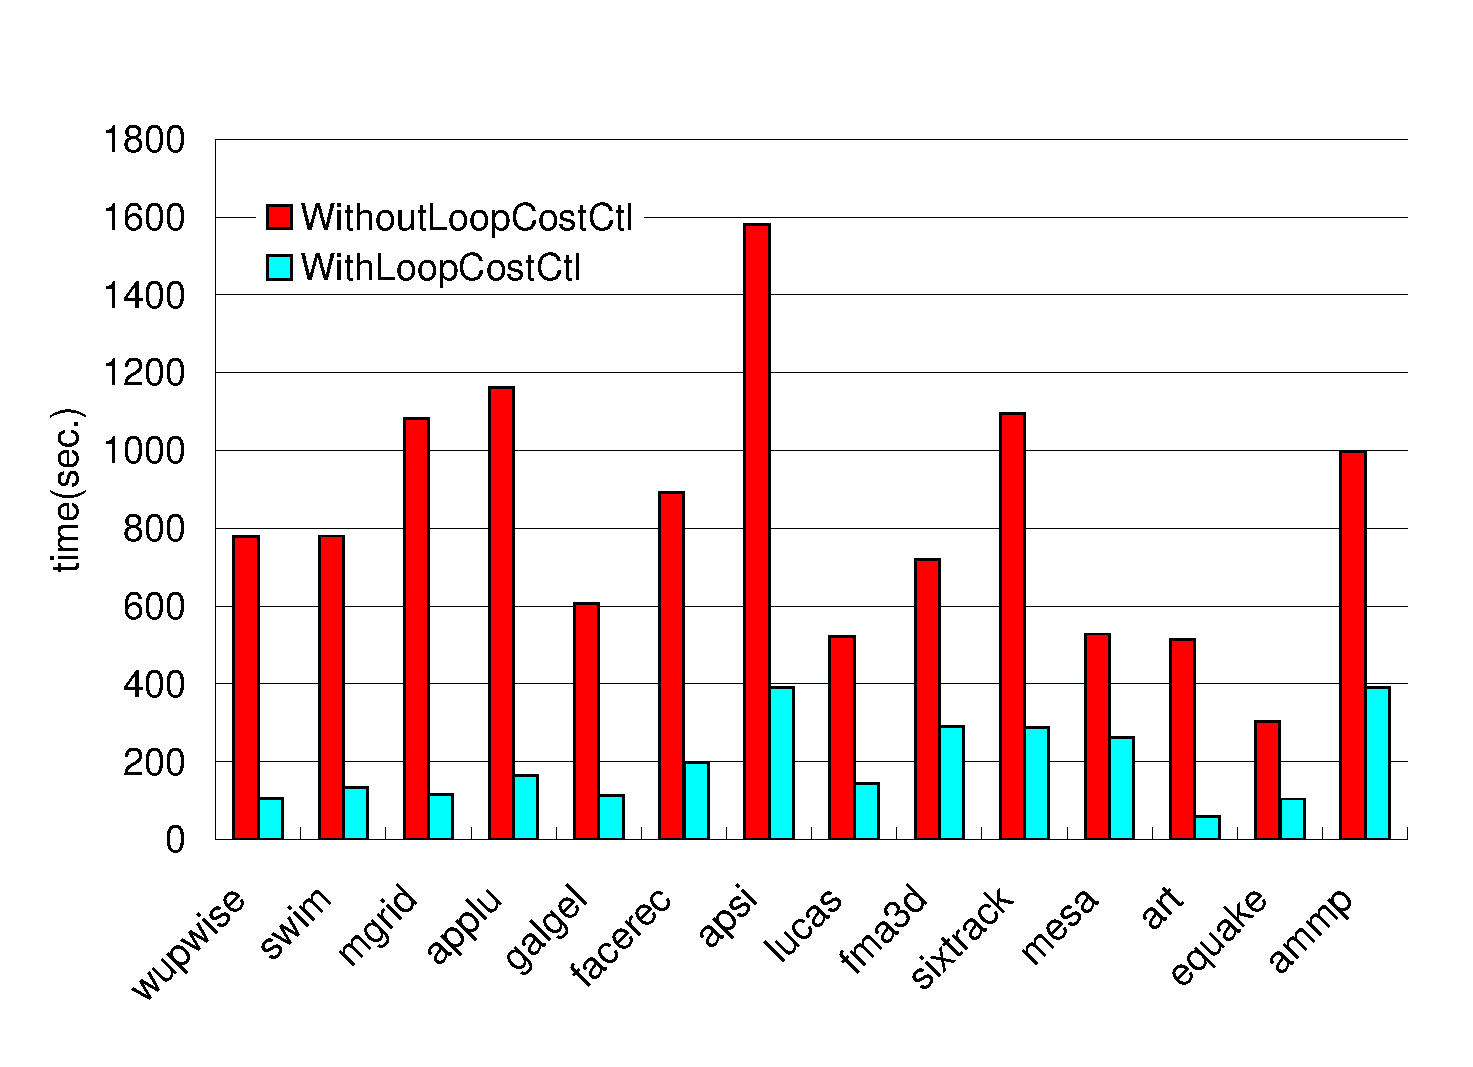
\includegraphics[angle=0, width=0.85\textwidth]{loopcost.eps}
    \caption{\footnotesize Benchmark performance with and without Loop Cost using two CPU's}
    \label{fig:loopcost_performance}
  \end{center}
\end{figure}


%\begin{table}
%\begin{center}
%\begin{tabular}{|l|c|c|} \hline
%\bf Benchmark & \bf Time(sec) & \bf Time(sec)\\
%& \bf Without Loop Cost & \bf With Loop Cost  \\
%\hline
%\hline
%swim & 780.18 & 134.56 \\ 
%\hline
%wupwise & 778.61 & 104.28 \\ 
%\hline
%mgrid & 1081.24 & 116.36\\
%\hline
%applu & 1161.56 & 163.92\\
%\hline
%galgel & 605.53 & 112.05\\
%\hline
%lucas & 522.34 & 142.92\\
%\hline
%mesa & 548.24 & 263.27\\
%\hline
%art & 513.68 & 60.10\\
%\hline
%equake & 302.97 & 103.98\\ 
%\hline
%ammp & 997.50 & 391.81 \\
%\hline
%apsi & 1581.05 & 390.63 \\
%\hline
%sixtrack & 1095.94 & 286.96 \\
%\hline
%fma3d & 720.80 & 291.52 \\
%\hline
%facerec & 891.11 & 196.63 \\
%\hline
%\end{tabular}
%\vspace{0.5cm}
%\caption{\label{loopcost_performance}Benchmark performance with and without Loop Cost}
%\end{center}
%\end{table}

% Enclosing tabular in a table ...compacts the table ie reduces the spacing between rows. It becomes Floating tables
\begin{table}
\begin{center}
\begin{tabular}{|l|c|c|c|c|c|} \hline
{\rule[-2mm]{0mm}{6mm}\bf Benchmark} & \bf \#Input Loops & \bf \#Loops Processed & \bf \#After Stage1 & \bf \#After Stage2/ & \bf\#After Stage3 \\
\hline
\multicolumn{6}{|c|}{\bf Stage1: Preliminary compile-time filtering }\\
\multicolumn{6}{|c|}{\bf Stage2: Compile-time loop cost filtering  }\\
\multicolumn{6}{|c|}{\bf Stage3: Runtime loop cost filtering  }\\
\hline
\hline
swim & 23 & 18 & 9 & 9 & 5\\
\hline
wupwise & 58 & 58 & 6 & 6 & 4\\ 
\hline
mgrid & 47 & 30 & 11 & 11 & 7\\ 
\hline
applu & 180 & 104 & 27 & 27 & 11\\ 
\hline
galgel & 642 & 538 & 280 & 280 & 36\\ 
\hline
lucas & 123 & 123 & 16 & 16 & 4\\ 
\hline
mesa & 777 & 777 & 118 & 118 & 0\\ 
\hline
art & 83 & 83 & 18 & 18 & 5\\ 
\hline
equake & 62 & 64 &  0 & 0 & 0\\ 
\hline
ammp & 283 & 282 & 18 & 18 & 0\\ 
\hline
apsi & 303 & 284 & 92 & 92 & 5\\ 
\hline
sixtrack & 1157 & 1135 & 347 & 347  & 11 \\ 
\hline
fma3d & 1648 & 1635 & 272 & 272 & 33\\ 
\hline
facerec & 202 & 133 & 69 & 69 & 9\\ 
\hline
\end{tabular}
\vspace{0.5cm}
\caption{\label{autopar_loops}Stages of Loop Selection for Auto-parallelization of Spec2000 FP Benchmarks}
\end{center}
\end{table}

\begin{table}
\begin{center}
\begin{tabular}{|l|c|c|c|c|} \hline
\bf Benchmark & \bf \#HighCostLoops & \bf \#Parallelizable & \bf \#HighCostLoops & \bf \#LowCostLoops \\
& \bf from PDF & \bf HighCostLoops& \bf selected by & \bf  selected by \\
& & \bf from PDF & \bf Parallelizer & \bf Parallelizer \\
\hline
\hline
swim & 8 & 5 & 5 & 0 \\
\hline
wupwise & 7 & 4 & 4 & 0 \\ 
\hline
mgrid & 9 & 7 & 7 & 0\\ 
\hline
applu & 41 & 11 & 11 & 0 \\ 
\hline
galgel & 84 & 49 & 36 & 0 \\ 
\hline
lucas & 47 & 4 & 4 & 0 \\ 
\hline
mesa & 74 & 3 & 0 & 0 \\ 
\hline
art & 37 & 5 & 5 & 0 \\ 
\hline
equake & 8 & 0 & 0 & 0 \\ 
\hline
ammp & 31 & 0 & 0 & 0 \\ 
\hline
apsi & 28 & 11 & 5 & 0 \\ 
\hline
sixtrack & 44 & 13 & 11 & 0 \\ 
\hline
fma3d & 61 & 33 & 33 & 0 \\ 
\hline
facerec & 43 & 25 & 9 & 0 \\ 
\hline
\end{tabular}
\vspace{0.5cm}
\caption{\label{autopar_accuracy}Evaluation of Loop Selection for Auto-parallelization of Spec2000 FP Benchmarks}
\end{center}
\end{table}

\subsection{Runtime Profiling}

In addition to using loop cost for restricting parallel loops, the auto-parallelizer employs runtime profiling\cite{Nan03} to further filter out
loops at a finer granularity. The runtime profiling is a more accurate
way of measuring the execution time of a chunk of code. The execution
time of a chunk of a loop executed in parallel (as measured by the
runtime profiler) is compared with selected \emph{serial} and
\emph{parallel} thresholds. If the execution time of the chunk is less
than the serial threshold, the next chunk of the loop is serialized
disregarding the decision from the runtime loop cost evaluation. The
decision to parallelize or serialize changes dynamically depending on
previous executions of the loop.



